\label{unit8}

% Search Menu

\section{Search Menu}

\begin{description}
\item [Find, Find Next, Find Previous] Via \textsf{Search}, you can find
and highlight residues in sequences. When you use \textsf{Find}, all of
the residues will be highlighted, and you can then cycle through them by
using \textsf{Find Next} and \textsf{Find Previous}.

\item[Select Contact Shells]
See Figure~\ref{fig:select_cs}.
 \begin{figure}[here]
 \centerline{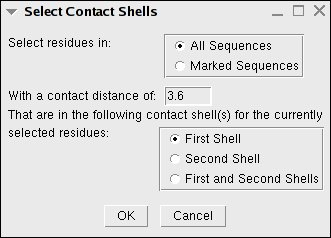
\includegraphics [width=3in]{./pictures/select_contactshells.jpg}}
 \caption{Select Contact Shell Window}
\label{fig:select_cs}
\end{figure}

\begin{description}
     \item[Select residues in:] Lets you choose whether to look through
     all sequences, or just the ones you have marked.
     \item[With a contact distance of:] defaults to 3.6.
     \item[That are in the following contact shell(s) for the currently
     selected residues] Choose from \textsf{First}, \textsf{Second}, or
     \textsf{First and Second} shells
\end{description}     

\item[Select Non-Redundant Set]

You can use structure QR or sequence QR to select a non-redundant set
(See Fig.~\ref{fig:select_nr}).

 \begin{figure}[here]
 \centerline{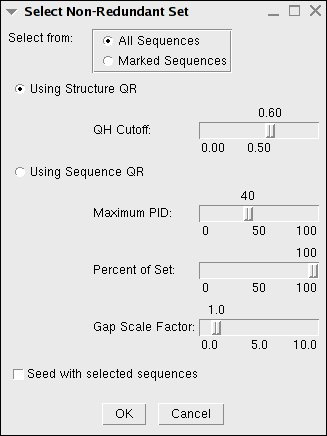
\includegraphics [width=3in]{./pictures/select_nrset.jpg}}
 \caption{Select Non-Redundant Set Window}
\label{fig:select_nr}
\end{figure}

% foobar.  Needs detail
\begin{description}
     \item[Select from:] Lets you choose whether to look through
     all sequences, or just the ones you have marked.
     \item[Using Structure QR]
          \begin{description}
               \item[QH Cutoff:]  Can vary from 0 to 1.
           \end{description}
    \item[Using Sequence QR]
             \begin{description}
               \item[Identity Cutoff:]
               \item[Gap Scale Factor:]
           \end{description}   
     \item[Seed with selected sequences]  If you have selected certain
     sequences, you can seed the algorithm with these sequences to
     select a non-redundant set based on them.
\end{description}

\item[Select Residues]
The \textsf{Residue Selection} feature (See
Fig.~\ref{fig:select_res})lets you analyze conservation, using different
measures, and highlight residues in the Sequence Display and Structure
Display simultaneously.  \textsf{Residue Selection} allows you to examine the
conservation on a per residue basis.
 
\begin{figure}[here]
\centerline{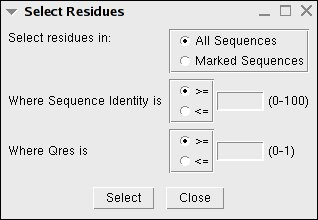
\includegraphics[width=3in]{./pictures/select_residues.jpg}}
\caption{Select Residues Window}%more information in caption about views
etc.  \label{fig:select_res} \end{figure}

There are two options: either \textsf{Where
Sequence Identity is} or \textsf{Where Qres is}.  \textsf{Where Sequence
Identity is} is a sequence identity measure, whereas \textsf{Where Qres
is} is a structure measure.

\begin{description}
     \item[Select residues in:] You can choose all sequences or just the
     marked ones.
     \item[Where Sequence Identity is:] If this option is selected you
     can select `less than or equal to' or `greater than or equal to' 
     option, then a number
     between 0-99.
     \item[Where Qres is:] If this option is selected you 
     can select `less than or equal to' or `greater than or equal to' 
     option, then a number between zero and one.
\end{description}
\end{description}

